\documentclass[12pt, a4paper]{article}

\usepackage[icelandic]{babel}
\usepackage[T1]{fontenc}

\usepackage{amsmath, amssymb, amsfonts}
\usepackage{mathtools}

\usepackage{minted}
\renewcommand{\listingscaption}{Forrit}

\usepackage{url}
\usepackage{hyperref}
\usepackage[hang, flushmargin]{footmisc}

\usepackage{xcolor}
\usepackage{tabularx}
\usepackage{graphicx}
\usepackage{booktabs}

\usepackage{fancyhdr}
\pagestyle{fancy}
\fancyhf{}
\fancyhead[L]{Kári Hlynsson}
\fancyhead[C]{TÖL203G HEIMADÆMI \#3}
\fancyhead[R]{\today}
\fancyfoot[C]{\thepage}

\newcommand{\doctitle}{\uppercase{Heimadæmi 3}}
\newcommand{\coursename}{Tölvunarfræði 2}
\newcommand{\coursenum}{TÖL203G}

% ——— Mengjatákn
\newcommand{\N}{\mathbb{N}}
\newcommand{\Z}{\mathbb{Z}}
\newcommand{\Q}{\mathbb{Q}}
\newcommand{\R}{\mathbb{R}}
\newcommand{\C}{\mathbb{C}}

% ——— Vigrar
\renewcommand{\u}{\mathbf{u}}
\renewcommand{\v}{\mathbf{v}}
\renewcommand{\b}{\mathbf{b}}
\newcommand{\w}{\mathbf{w}}
\newcommand{\p}{\mathbf{p}}
\newcommand{\x}{\mathbf{x}}
\newcommand{\y}{\mathbf{y}}
\newcommand{\z}{\mathbf{z}}

\title{}

\begin{document}
\thispagestyle{plain}
\centerline{\bfseries\Large\doctitle}
\medskip
\centerline{\large\coursenum\ \coursename}
\bigskip

\centerline{\large Kári Hlynsson}
\bigskip
\centerline{Háskóli Íslands}
\medskip
\centerline{\today}

\bigskip

\noindent
\textbf{\large Verkefni 1} \medskip \\
Breytið \texttt{FourSum.java} í \texttt{FourSumFast.java} á sama hátt og er
gert með \texttt{ThreeSumFast.java}. Skilið kóða fallsins \texttt{count}
(sem texta, ekki skjáskoti) og skjáskoti af keyrslu \texttt{FourSum} og
\texttt{FourSumFast} á gagnaskránni 1Kints.txt. Þá eiga að finnast 13654
ferndir. Athugið að þið þurfið að laga kóðann aðeins, því texttt{FourSum.java}
notar \texttt{long} fylki í stað \texttt{int} fylkis og innlestur gagnanna er aðeins ólíkur.

\medskip
\noindent
\textbf{\large Lausn} \medskip \\
Breytingarnar eru lítillegar og sjást fyrir neðan í forriti \ref{forrit1}.

\begin{listing}[ht!]
    \centering
    \inputminted[firstline=49, lastline=65, linenos]{java}{../src/FourSumFast.java}
    \caption{Fallið \texttt{count} í \texttt{FourSumFast.java}}
    \label{forrit1}
\end{listing}

\noindent
Mynd \ref{mynd1} sýnir keyrslu í skel á \texttt{FourSum.java} og síðan \texttt{FourSumFast.java}.

\begin{figure}[ht!]
   \centering
   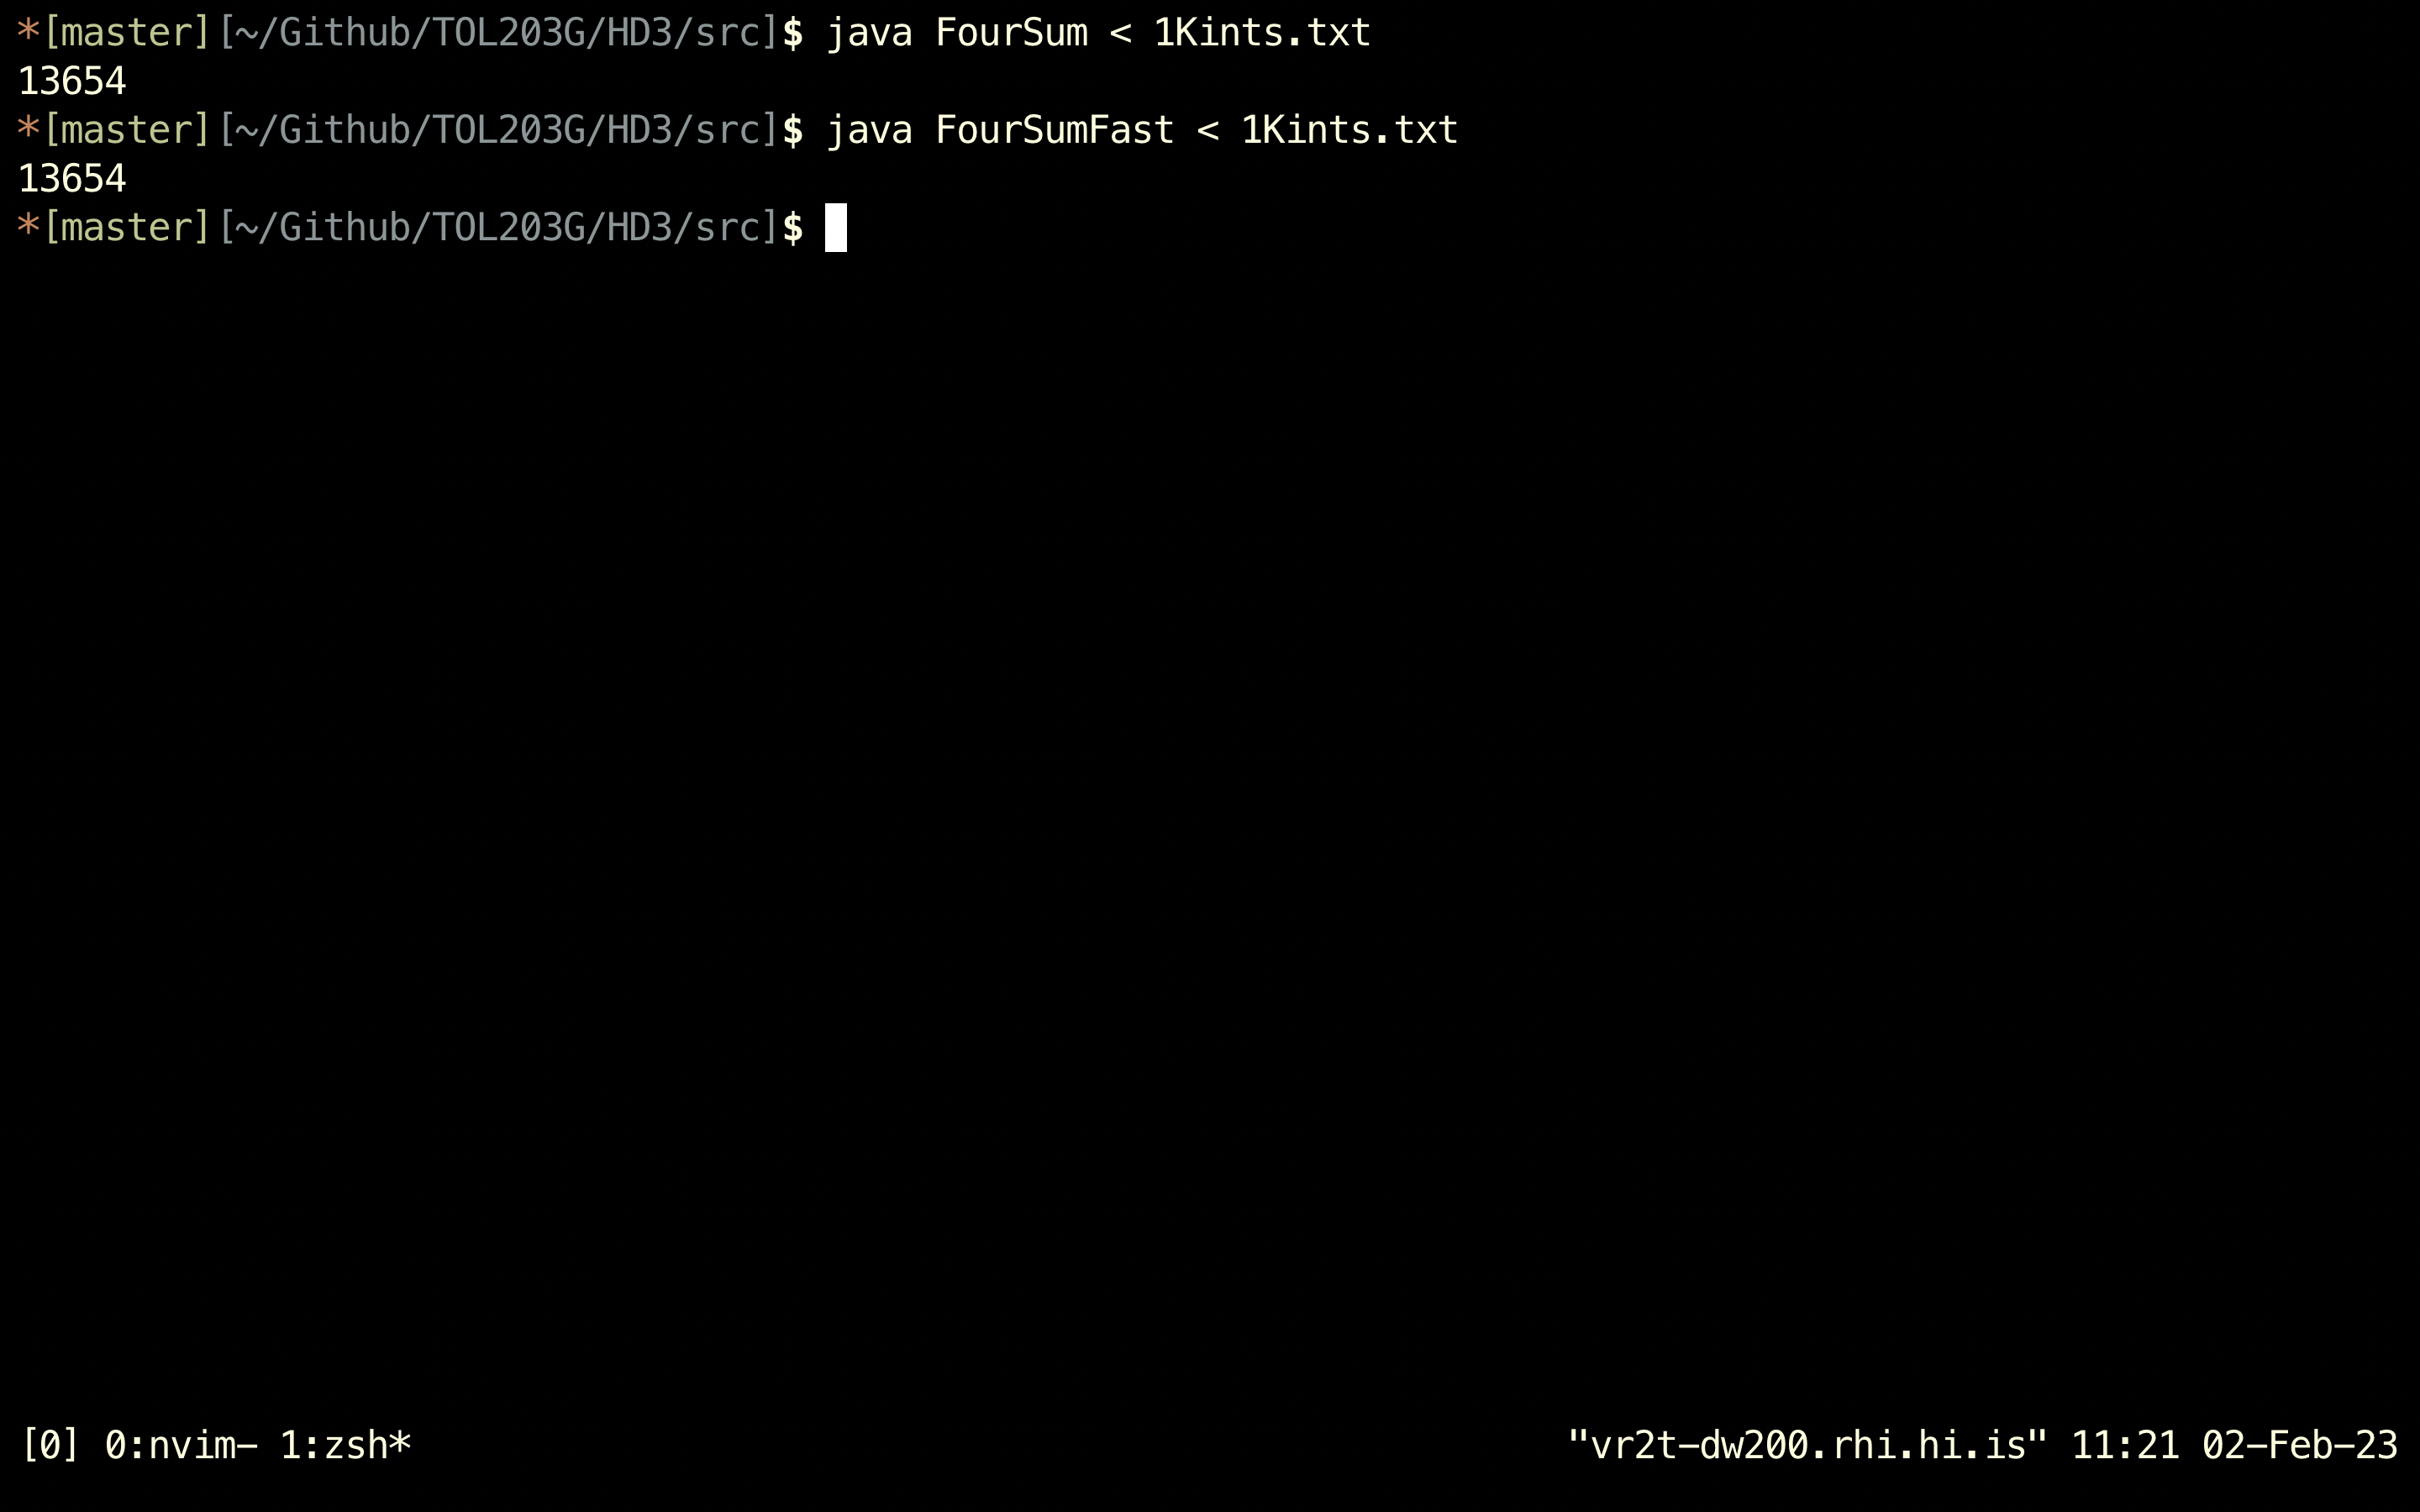
\includegraphics[width=\textwidth]{img/foursum_keyrsla.png} 
   \caption{Keyrsla \texttt{FourSum} og \texttt{FourSumFast} í skel}
   \label{mynd1}
\end{figure}

\end{document}